%------------------------ Packages ------------------------
\documentclass[12pt,a4paper]{article}
\usepackage[latin1]{inputenc}
\usepackage[T1]{fontenc}
\usepackage[pdftex]{graphicx}
\usepackage{float}
\usepackage{amsmath}
\usepackage{amssymb}
\usepackage[FIGTOPCAP]{subfigure}
\usepackage{color}
\usepackage[hidelinks]{hyperref}

\newcommand{\version}{\IfFileExists{../../version.txt}
{\input{../../version.txt}}
{\input{../../../version.txt}}
}

\newcommand{\command}[1]{%
\indent \fcolorbox{black}{white}{%
   \begin{minipage}{\dimexpr\textwidth-\parindent\relax}%
      #1
   \end{minipage}%
}
}

\newsavebox{\FVerbBox}
\newenvironment{sample}
{\par \vspace{0.2cm} \begin{lrbox}{\FVerbBox}
\begin{minipage}{\dimexpr\textwidth-\parindent\relax}}
{\end{minipage}
\end{lrbox}
\fcolorbox{black}{lightgray}{\usebox{\FVerbBox}}
\vspace{0.2cm}}

\newenvironment{sampletitle}
{\vspace{0.2cm} \noindent\textbf{Example} :
\begin{sample}}
{\end{sample}}

\newcommand{\samplecomment}[1]{%

\textit{#1}
}

\newcommand{\seealso}[1]{\vspace{0.2cm} \noindent\textbf{See also} :\par #1}

% tikz
\usetikzlibrary{calc}
\usetikzlibrary{arrows}
\usetikzlibrary{shadows}

\tikzset{block/.style={draw, text centered, fill=gray!10,drop shadow}}
\tikzset{connect/.style={draw, line width=1 pt}}

\begin{document}

\begin{center}
\textbf{\huge  \underline{Dynroi operator}}
\end{center}
\vspace{0.5cm}

The dynroi operator is a morphological operation on a binary image used to create a binary mask. This operator detects the largest area of interest, i.e. the smallest rectangle which includes all non-black pixels, and outputs a black image with a white rectangle on this ROI coordinates. \\

\begin{figure}[h!]
\centering
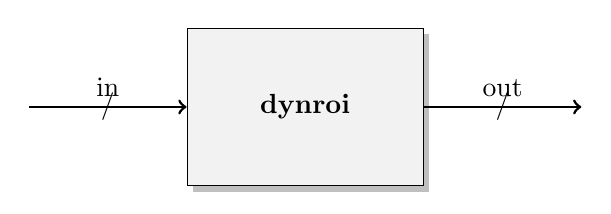
\begin{tikzpicture}
\node[block,rectangle,minimum height=2cm,minimum width=3cm] (bloc) {\textbf{dynroi}};

\path[connect,<-] ([yshift=0.0cm]bloc.west) -- node{/} node[above]{in} ++(-2cm,0);

\path[connect,->] ([yshift=0.0cm]bloc.east) -- node{/} node[above]{out} ++(2cm,0);
 ([xshift=0.5cm,yshift=-0.6cm]bloc.north);

\end{tikzpicture}
\end{figure}

This operator includes two differents operations:
\begin{itemize}
\item A selection of the image output: If the processed pixel is in the region of interest, the output will be a white pixel, otherwise a black pixel will be the output. If the bypass option is checked, no selection occurs and the block acts as a wire.
\item Update of region of interest coordinates: the minima and maxima for non black pixels coordinates are saved for one image and processed into a rectangle form (x,y,width,height) which is the region of interest of the next image. This computing is based on the assumption of a low difference between two consecutive images.
\end{itemize}


\vspace{0.5cm}

\begin{figure}[!h]
\centering
\subfigure[Initial greyscale image]{
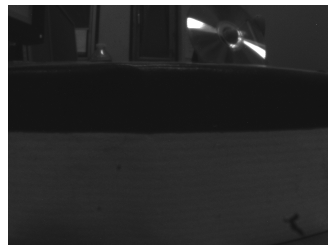
\includegraphics[width=9cm]{original.png}}
\hspace{2cm}
\subfigure[Binarized image]{

\includegraphics[width=9cm]{binary.png}}
\vspace{1cm}
\subfigure[Output with area of interest]{

\includegraphics[width=9cm]{result.png}}
\end{figure}

\section*{Properties}
\properties{
enable           & bool & Enable the processing (no output) \\ 
bypass           & bool & Bypass the processing (act as a wire)\\ 
}

\vspace{0.5cm}

\section*{Constants}

\constants{
CLK\_PROC\_FREQ & Frequency clock of the process \\
IN\_SIZE & Size of the input flow : 1 byte (greyscale image) or 1 bit (binary image)\\
OUT\_SIZE & Size of the output flow : 1 byte (greyscale image) or 1 bit (binary image)\\
}




\end{document}